%!TEX root = ../../master.tex

\subsection*{Application Layer}
The two previous sections described how Kubernetes runs and manages containerized applications (Figure~\ref{fig:flow_spring_software}). Now we will focus on the applications running on top of the infrastructure.
The application layer is not limited to a single language or framework since Docker containers are used. In order to experiment with microservices, a microservice chassis framework is chosen: Spring Boot and Spring Cloud. These frameworks make it easy to get up and running with a microservice architecture in Java. Furthermore, Spring Boot and Spring Cloud offer many relevant cloud computing libraries that easily can be included in projects. Multiple Netflix Open Source libraries are accessible through Spring Cloud e.g. an implementation of a circuit breaker for synchronous communication (Hystrix) and an implementation of the API Gateway pattern (Zuul). These libraries and examples of implementing them are described in further details in Appendix~\ref{appendix:application_layer}. \\


\noindent
KubeCloud is used as a presentation item as well as a practice item. In order to accommodate the role as a presentation item a demo project demonstrating some concepts of microservices, Docker and Kubernetes has been implemented. Secondly, the demo project supports the role as a practice item by providing a reference point for the students to get started. The demo project is a simplified microservice architecture to keep the initial complexity and understanding of the system low. The architecture contains four services as depicted in Figure~\ref{fig:demo}.

\begin{figure}[H]
    \centering
    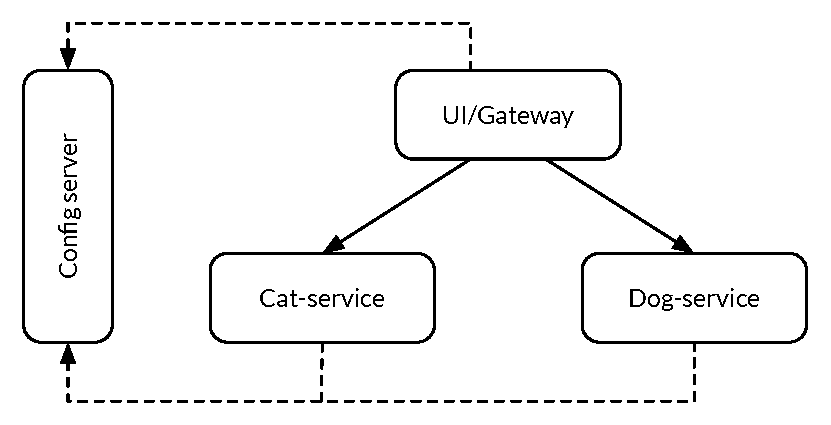
\includegraphics[width=9cm]{figures/demo_architecture}
    \caption{Architecture of Demo Application}
    \label{fig:demo}
\end{figure}

\noindent The four services are:
\begin{itemize}
  \item \textbf{Config-server}: The config server is implemented with the Spring Cloud Config, and acts as a central configuration management hub.
  \item \textbf{UI/Gateway}: The UI/Gateway is an implementation of the API Gateway pattern along with the graphical user interface (GUI) of the application.  
  \item \textbf{Cat-service}: The cat-service is a RESTful service, returning a list of cat-objects 
  \item \textbf{Dog-service}: The dog-service is a RESTful service, returning a list of dog-objects.
\end{itemize}

\noindent 
The graphical user interface makes requests to the API Gateway that then directs the calls to the specific service. The application is shown in Figure~\ref{fig:example} in which the data from cat-service is shown in Figure~\ref{fig:example}(b).

\begin{figure}[H]%
    \centering
    \subfloat[UI Gateway]{{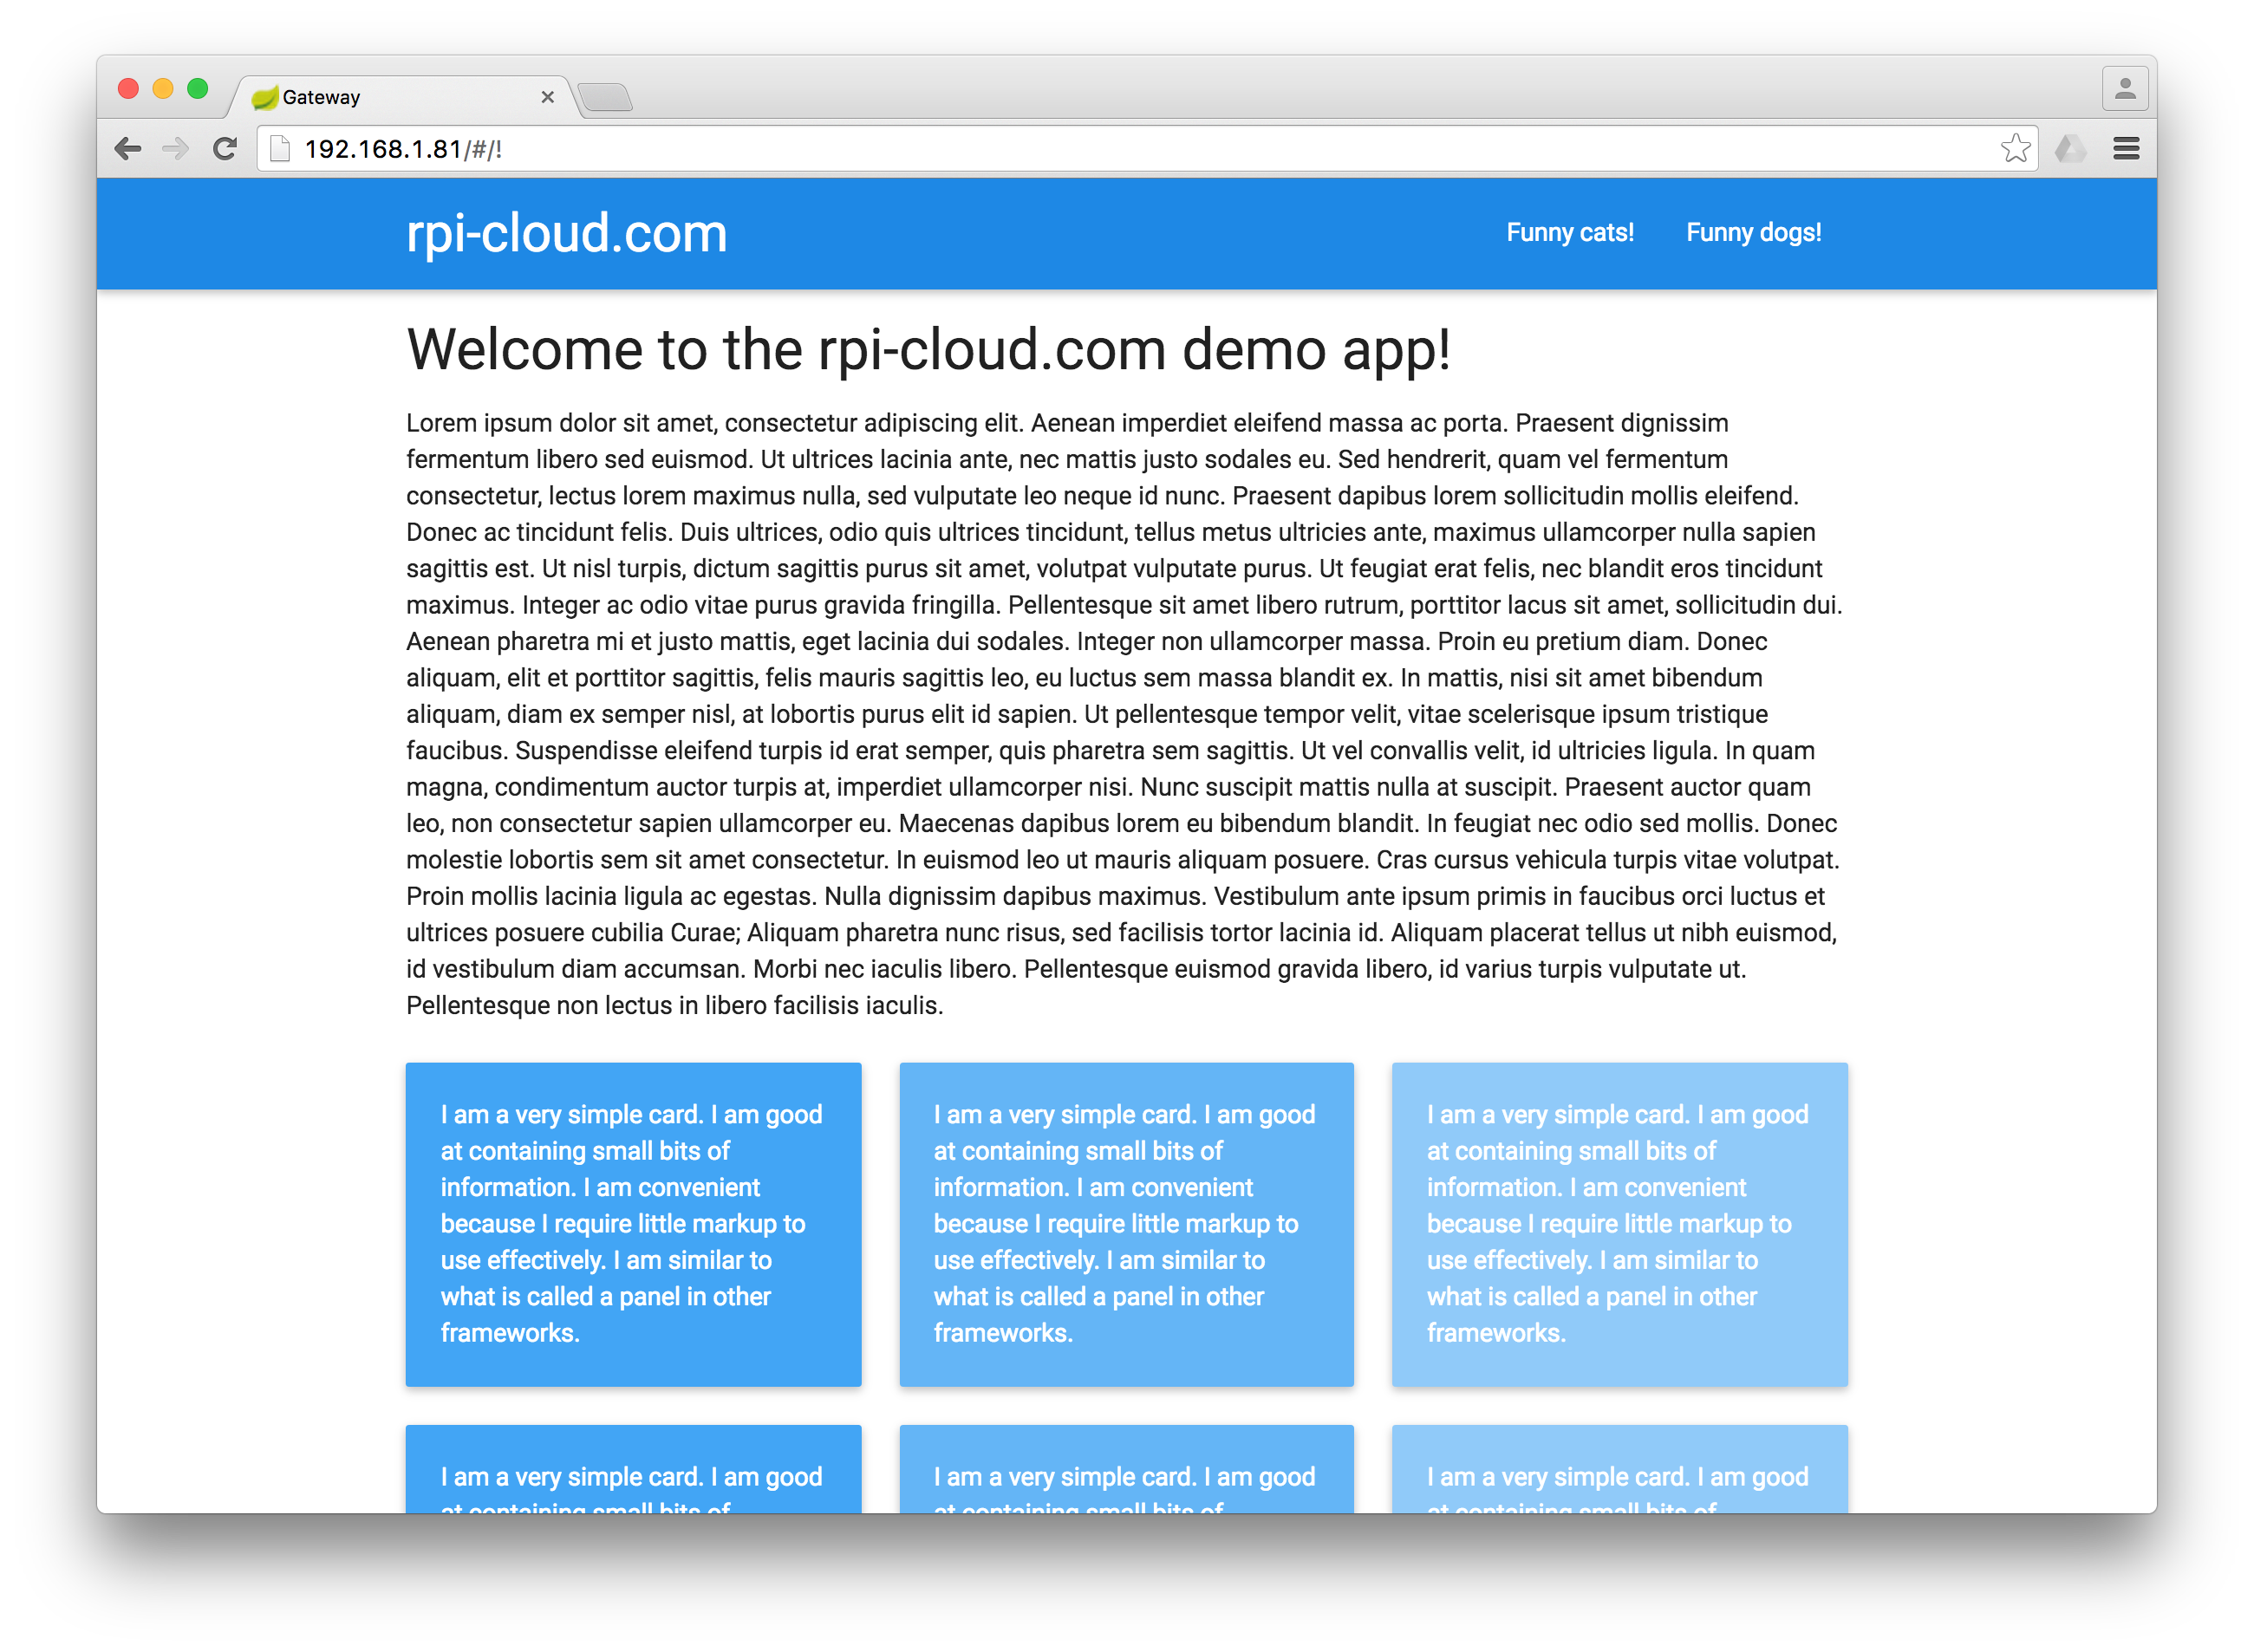
\includegraphics[width=7cm]{figures/demo/home} }}%
    \qquad
    \subfloat[Cats v2]{{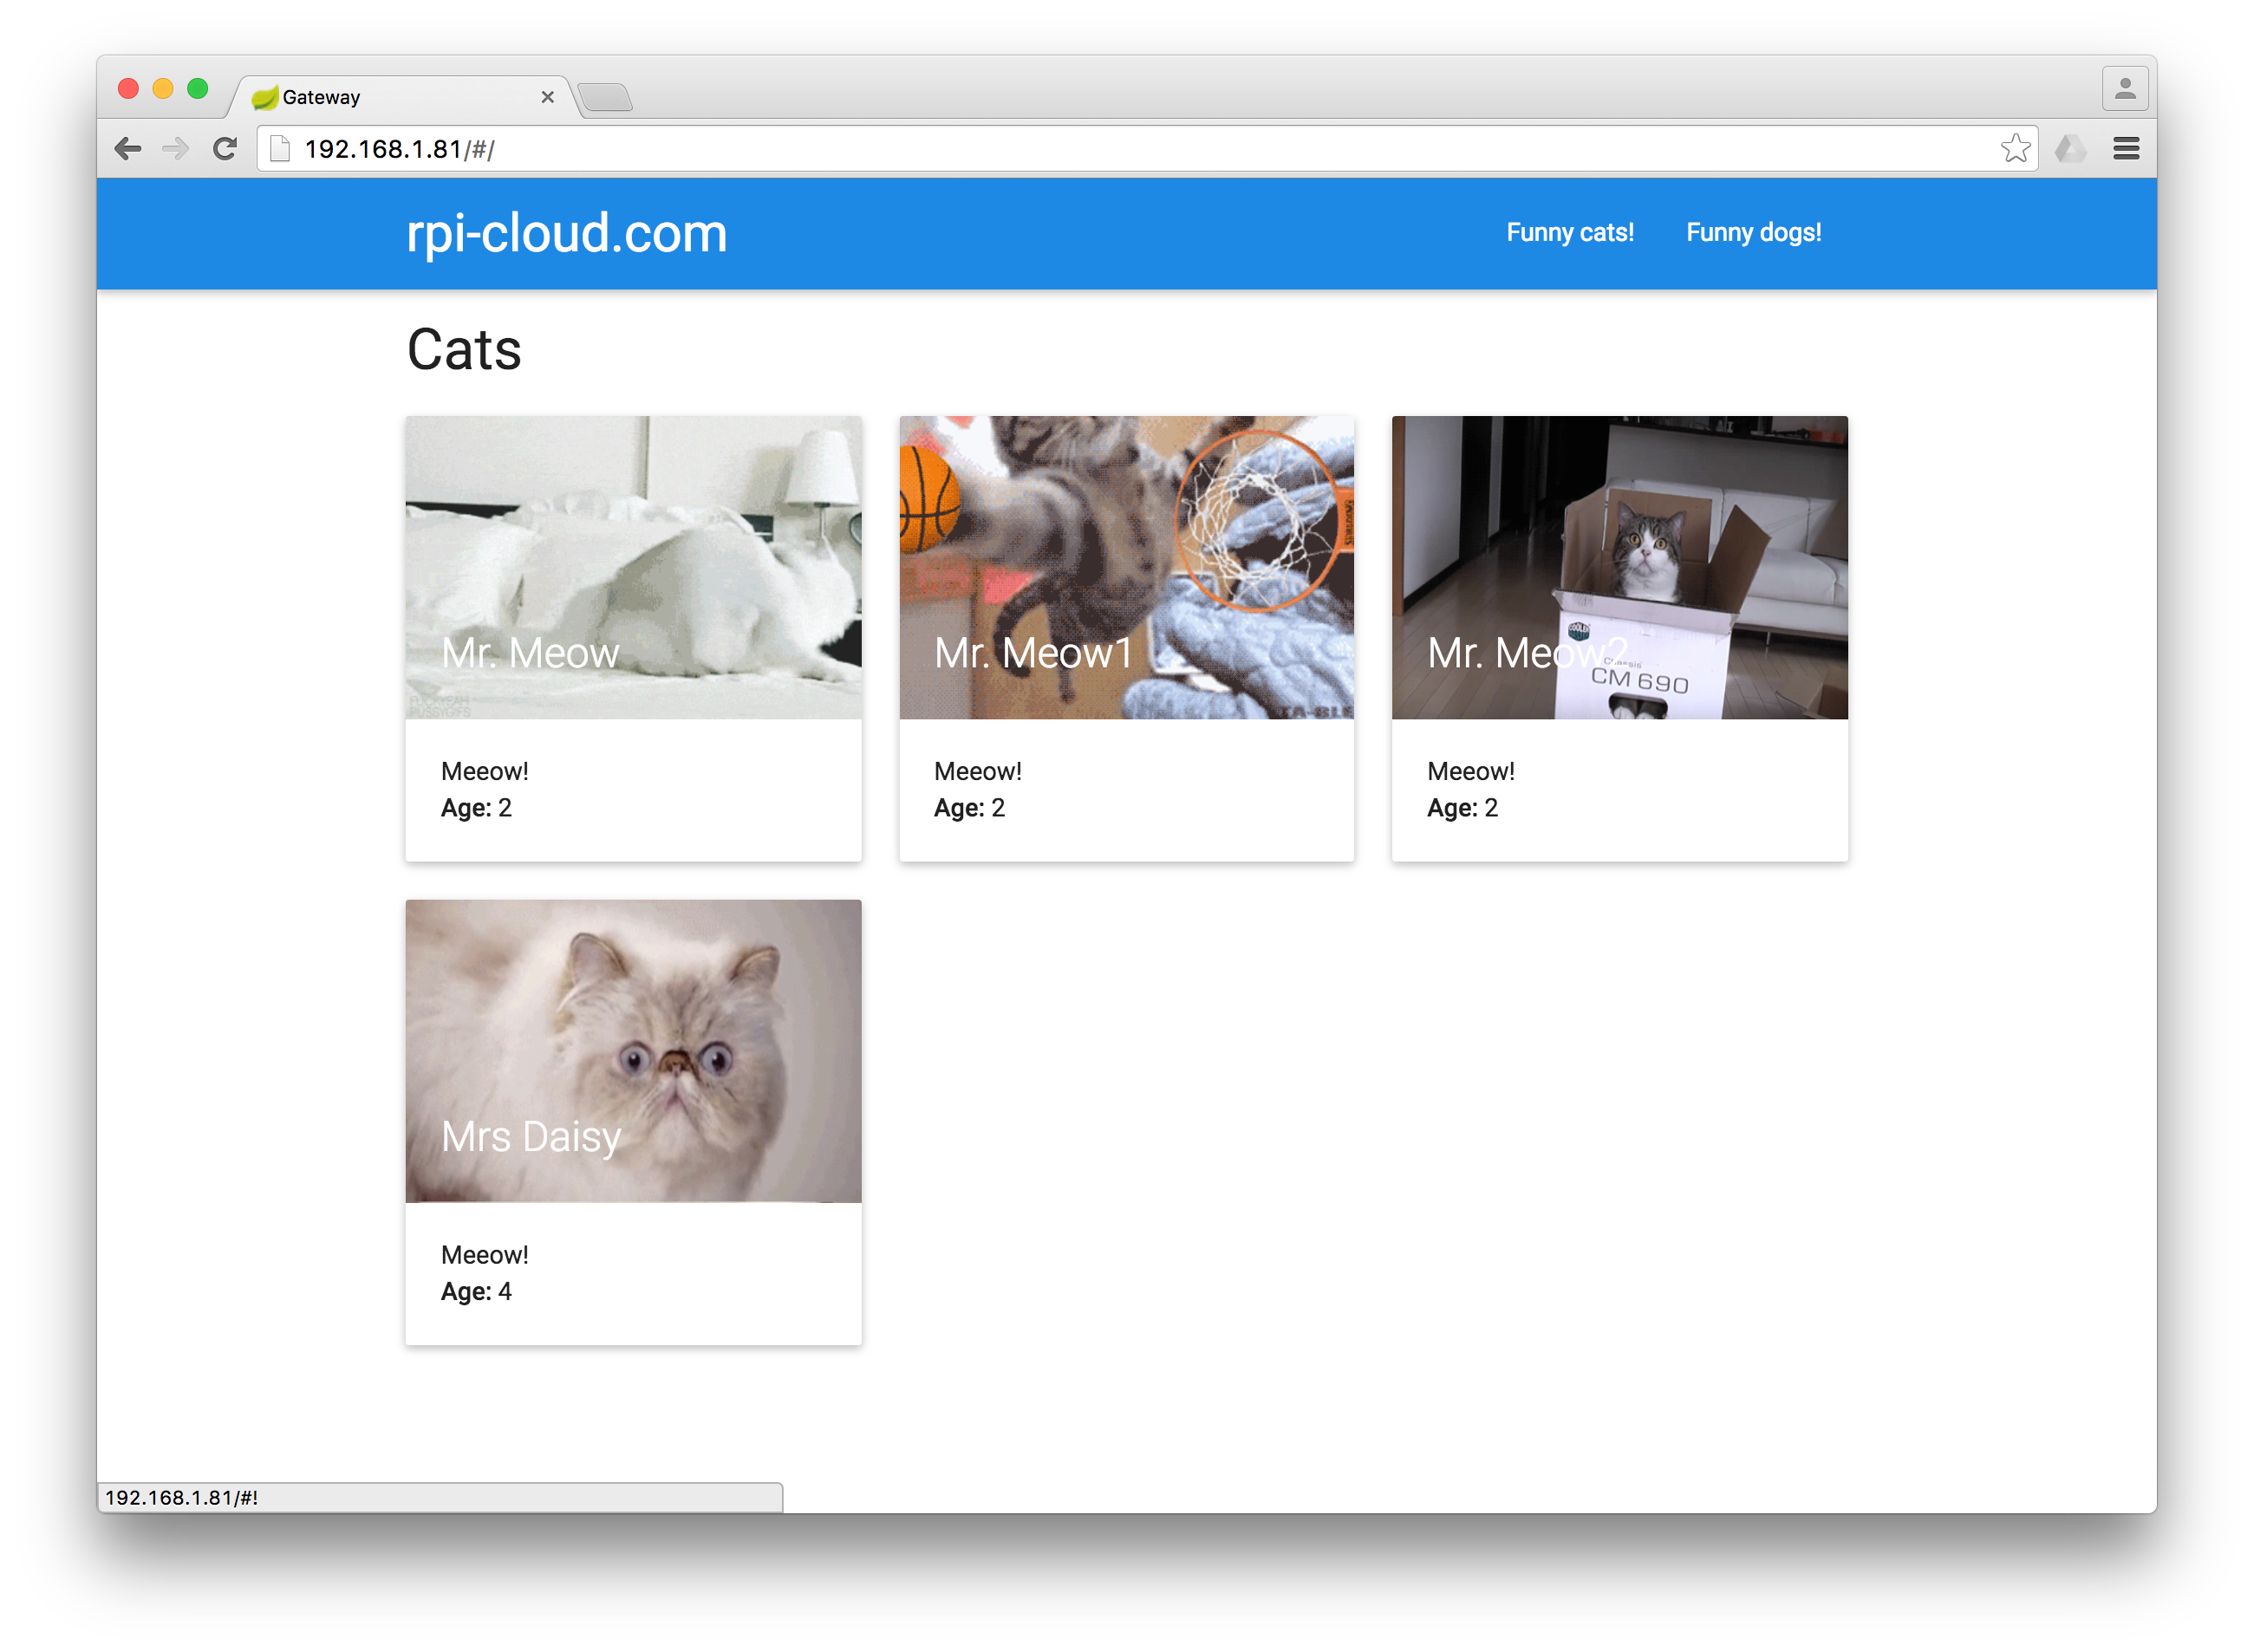
\includegraphics[width=7cm]{figures/demo/cats_v2} }}%
    \caption{Screenshots of Demo Application}%
    \label{fig:example}%
\end{figure}

\noindent
The previously mentioned DNS add-on for Kubernetes is used for service discovery for the individual microservices in this dynamic environment. The DNS add-on allows inter-service communication by using the Kubernetes services' names instead of IPs. Figure~\ref{fig:dns} shows an example where a service makes a request to \textbf{http://config-service}. This service name will then be attempted resolved on the host by looking up the designated DNS services. The resolv.conf file, from the host machine, contains the IPs of the DNS services. The KubeDNS virtual IP is added to resolv.conf by kubernetes-on-arm. KubeDNS is then contacted and looks up \textbf{config-service} in etcd. If found, the resolved IP will be sent back, and the service name is resolved to a virtual IP that the request is sent to as specified in Figure~\ref{fig:flannel}. 

\begin{figure}[H]
    \centering
    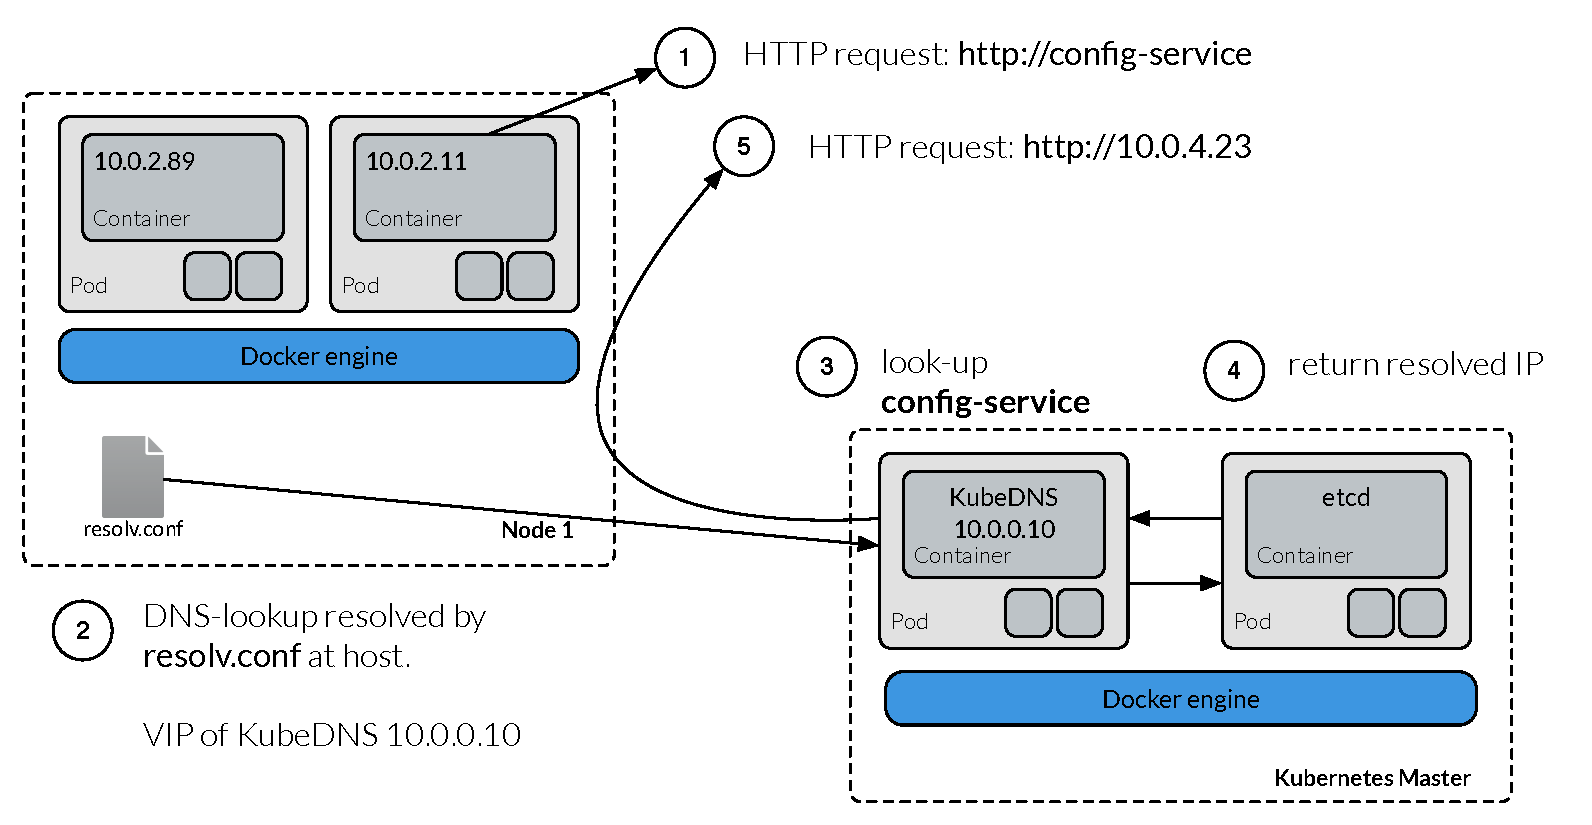
\includegraphics[width=12cm]{figures/kubernetes/kubedns}
    \caption{KubeDNS}
    \label{fig:dns}
\end{figure}